\section{Analisi e benchmark}

Per verificare che i metodi si comportassero in maniera corretta, abbiamo provato ad eseguire da interfaccia grafica una serie di test.
Le seguenti analisi nascono dai dati ricavati dall'esecuzione dei quattro metodi iterativi, i parametri considerati sono: \textit{tolleranza utilizzata} durante la fase di risoluzione, il \textit{tempo di esecuzione espresso in millisecondi}, il \textit{numero di iterazioni} effettuate per arrivare all'output, l'\textit{errore relativo} della soluzione ottenuta in relazione a quella di partenza e il \textit{nome della matrice risolta}. Il fine è quello di avere un'idea molto generale sul funzionamento dei metodi sui vari tipi di matrici.

\paragraph{Tolleranza vs errore relativo}
Abbiamo pensato di mettere in relazione l'errore relativo e la tolleranza utilizzata in fase di risoluzione dei quattro metodi a paragone; l'obiettivo è stabilire in che modo, al variare della tolleranza, il valore dell'errore relativo dei metodi potrebbe differire. In Figura \ref{fig:tolerrmat} e \ref{fig:tolerrmet} sono presenti i grafici relativi alla relazione tra tolleranza ed errore, raggruppati, rispettivamente, per matrici e per metodi.



\begin{figure}%
	\centering
	\subfloat{{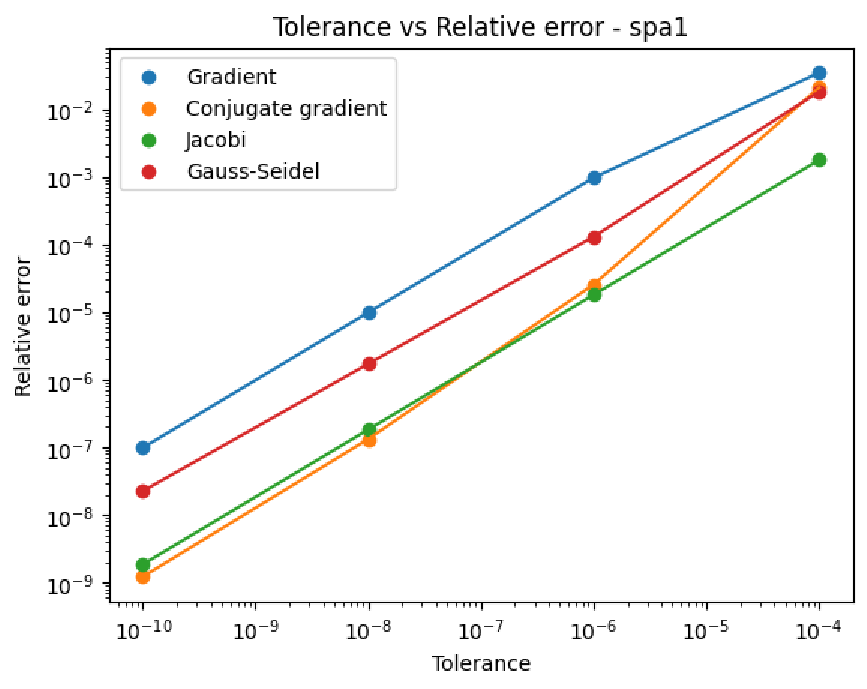
\includegraphics[width=0.40\textwidth]{figures/Tolerance vs Relative error/Difference between the 4 methods/spa1.pdf} }}%
	\subfloat{{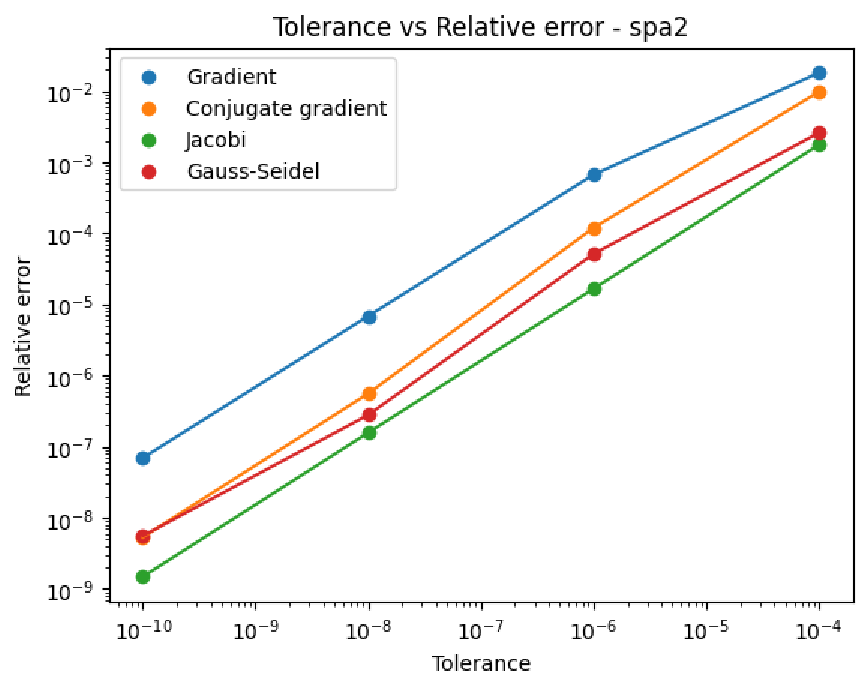
\includegraphics[width=0.40\textwidth]{figures/Tolerance vs Relative error/Difference between the 4 methods/spa2.pdf} }}%
	\qquad
	\subfloat{{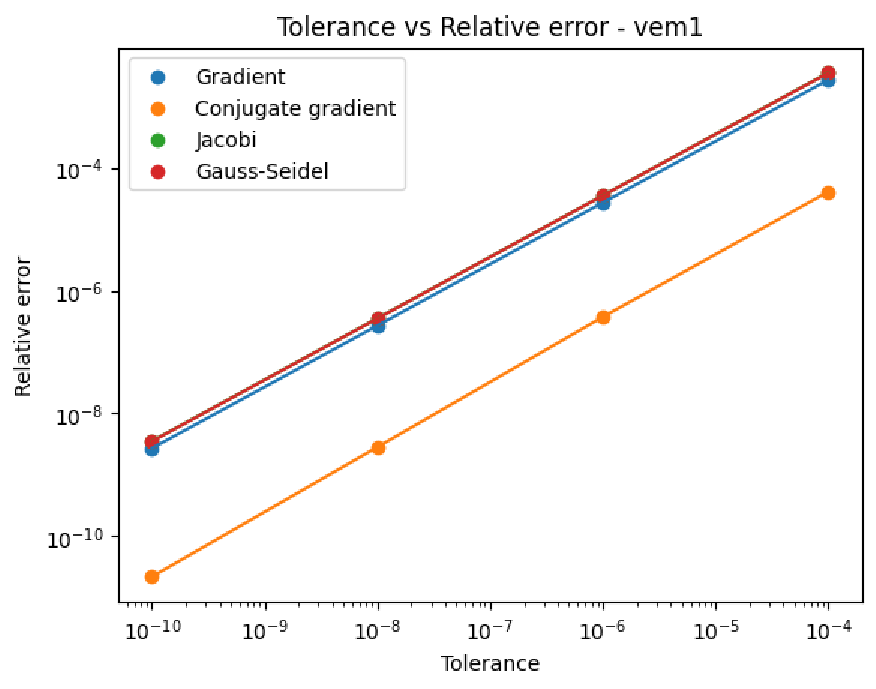
\includegraphics[width=0.40\textwidth]{figures/Tolerance vs Relative error/Difference between the 4 methods/vem1.pdf} }}%
	\subfloat{{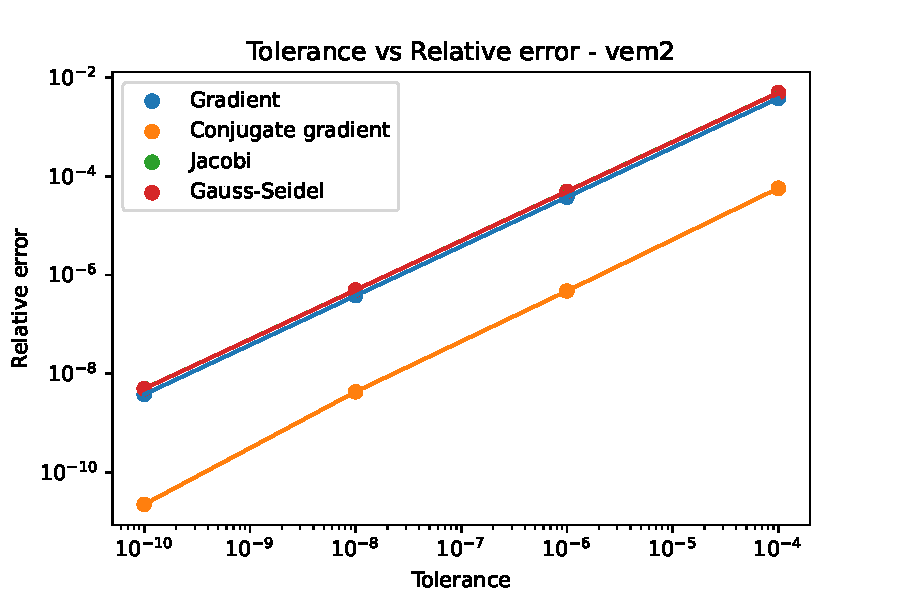
\includegraphics[width=0.40\textwidth]{figures/Tolerance vs Relative error/Difference between the 4 methods/vem2.pdf} }}%
	\caption{Grafici tolleranza / errore relativo sulle varie matrici di benchmark}%
	\label{fig:tolerrmat}
\end{figure}


\begin{figure}%
	\centering
	\subfloat{{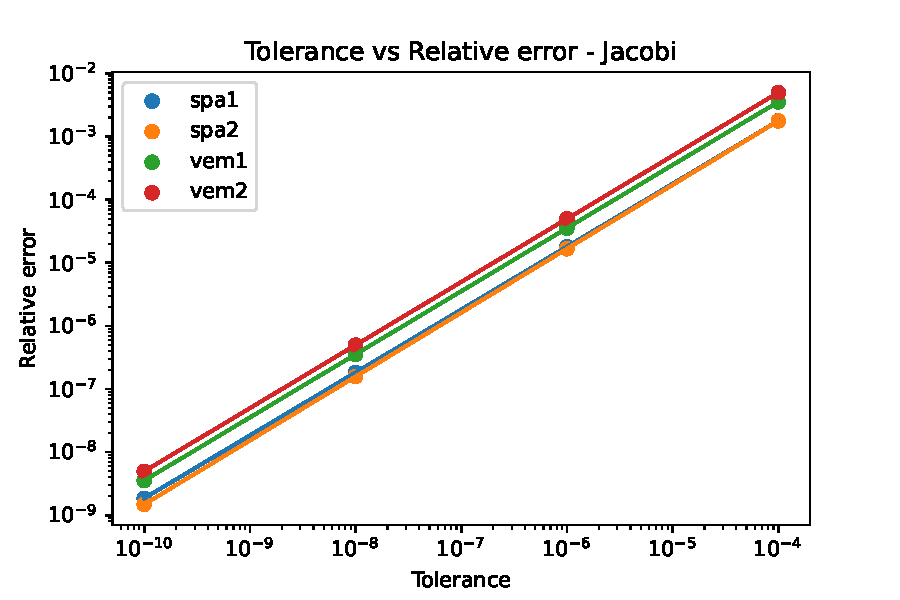
\includegraphics[width=0.40\textwidth]{figures/Tolerance vs Relative error/Difference between the 4 matrices on the same method/Jacobi.pdf} }}%
	\subfloat{{\includegraphics[width=0.40\textwidth]{figures/Tolerance vs Relative error/Difference between the 4 matrices on the same method/Conjugate Gradient.pdf} }}%
	\qquad
	\subfloat{{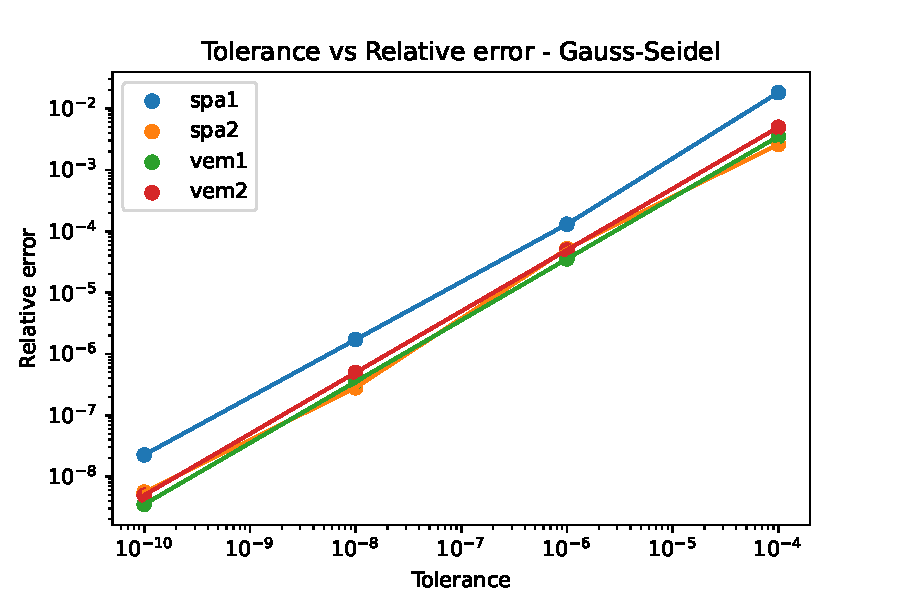
\includegraphics[width=0.40\textwidth]{figures/Tolerance vs Relative error/Difference between the 4 matrices on the same method/Gauss-Seidel.pdf} }}%
	\subfloat{{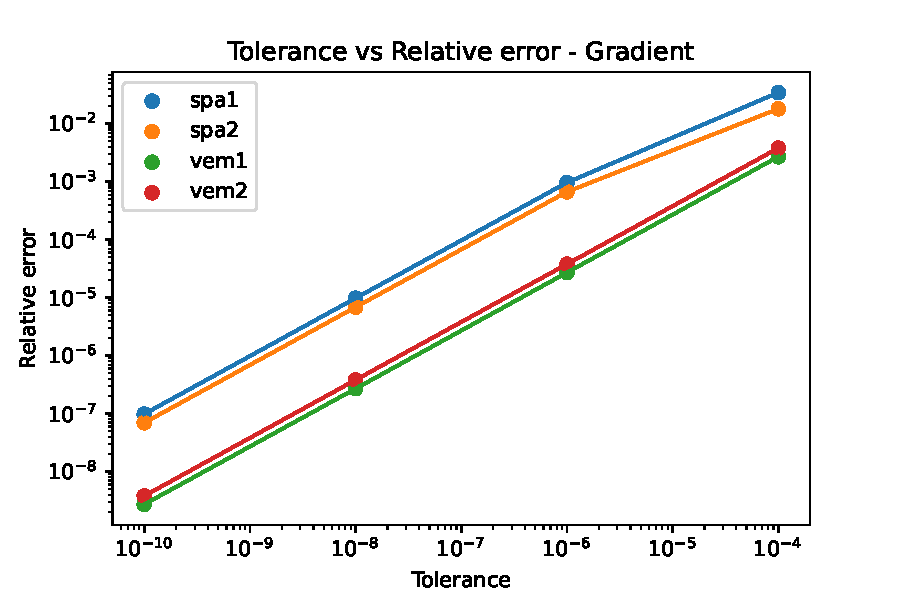
\includegraphics[width=0.40\textwidth]{figures/Tolerance vs Relative error/Difference between the 4 matrices on the same method/Gradient.pdf} }}%
	\caption{Grafici tolleranza / errore relativo rispetto i singoli metodi}%
	\label{fig:tolerrmet}
\end{figure}
%Immagine tolerance-relative_error, spa1, difference between the 4 methods
%Immagine tolerance-relative_error, spa2, difference between the 4 methods
%Immagine tolerance-relative_error, vem1, difference between the 4 methods
%Immagine tolerance-relative_error, vem2, difference between the 4 methods


Osservando i grafici, l'incremento dell'errore relativo è direttamente proporzionale alla crescita della tolleranza utilizzata durante l'esecuzione dei quattro metodi. Il risultato è ragionevole, così come indicato al capitolo \ref{tol/time, diff methods}, all'aumentare della tolleranza il criterio di arresto sarà meno restrittivo, portando ad una soluzione meno accurata, ergo ad un aumento dell'errore relativo.

\paragraph{Tolleranza vs tempo trascorso}\label{tol/time, diff methods}


\begin{figure}%
	\centering
	\subfloat{{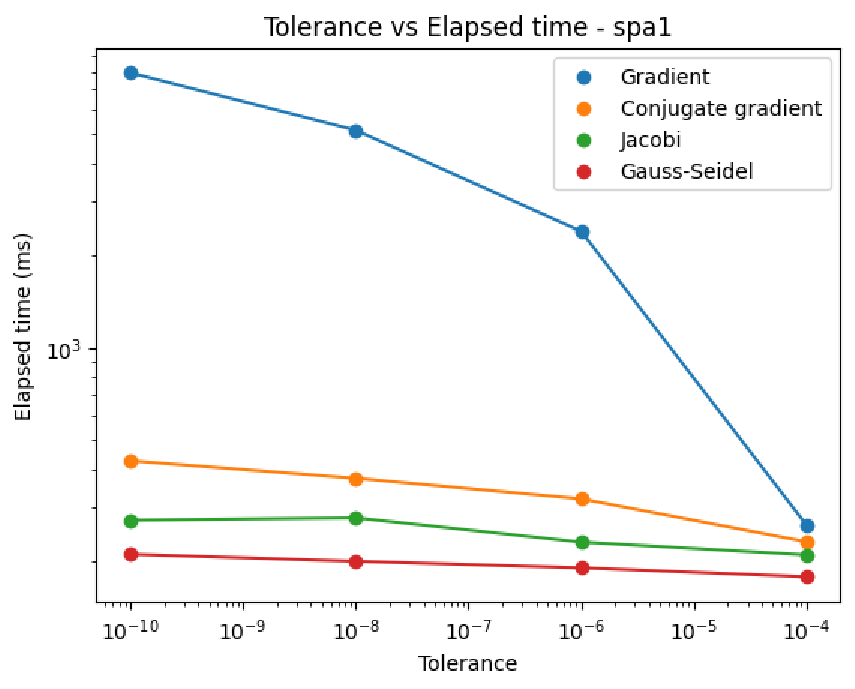
\includegraphics[width=0.40\textwidth]{figures/Tolerance vs Elapsed time/Difference between the 4 methods/spa1.pdf} }}%
	\subfloat{{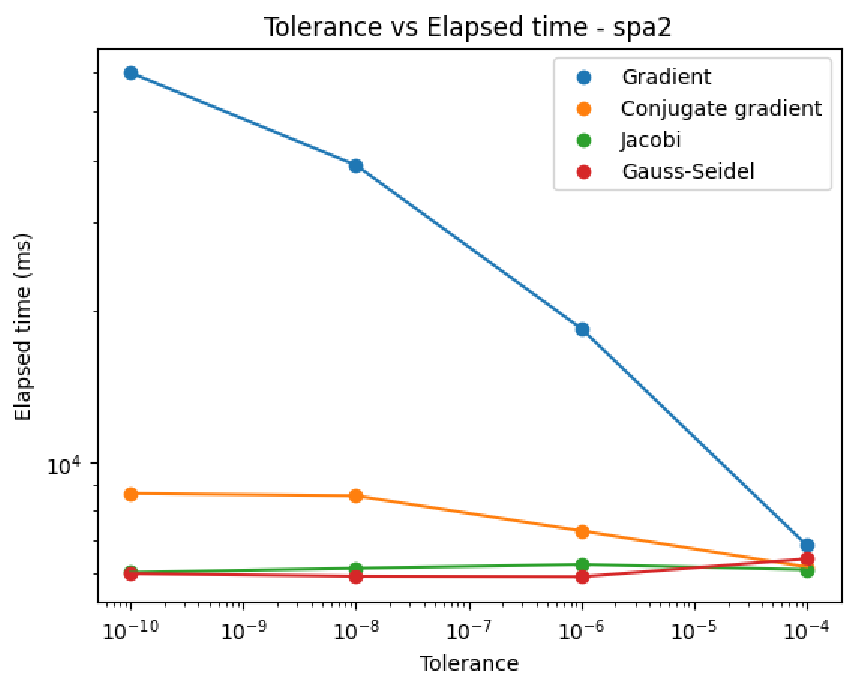
\includegraphics[width=0.40\textwidth]{figures/Tolerance vs Elapsed time/Difference between the 4 methods/spa2.pdf} }}%
	\qquad
	\subfloat{{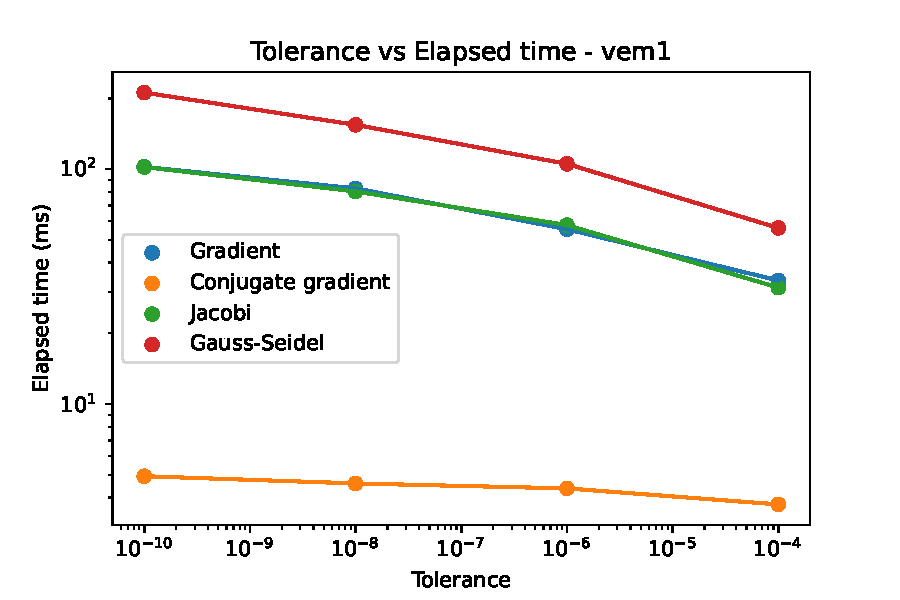
\includegraphics[width=0.40\textwidth]{figures/Tolerance vs Elapsed time/Difference between the 4 methods/vem1.pdf} }}%
	\subfloat{{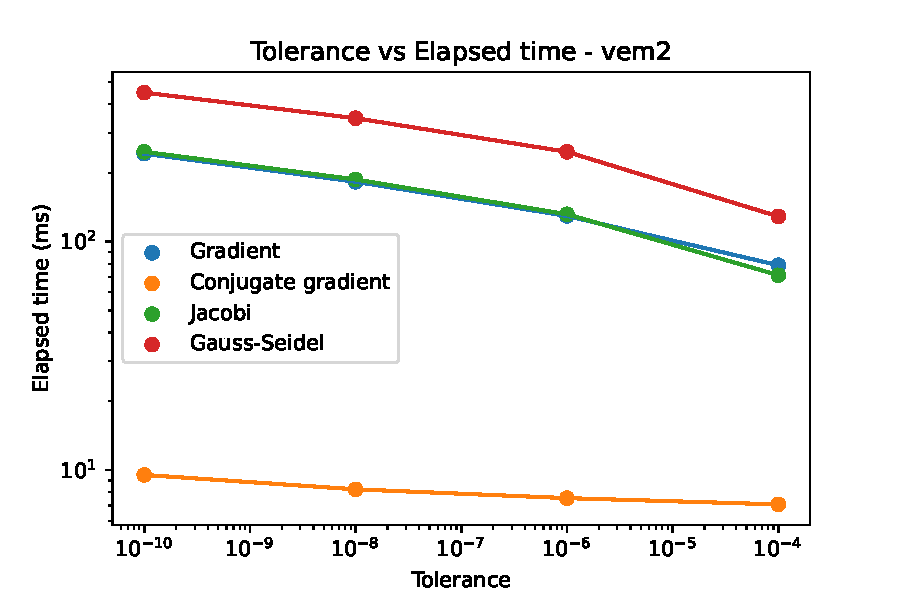
\includegraphics[width=0.40\textwidth]{figures/Tolerance vs Elapsed time/Difference between the 4 methods/vem2.pdf} }}%
	\caption{Grafici tolleranza / tempi sulle varie matrici di benchmark}%
	\label{fig:toltimemat}
\end{figure}

\begin{figure}%
	\centering
	\subfloat{{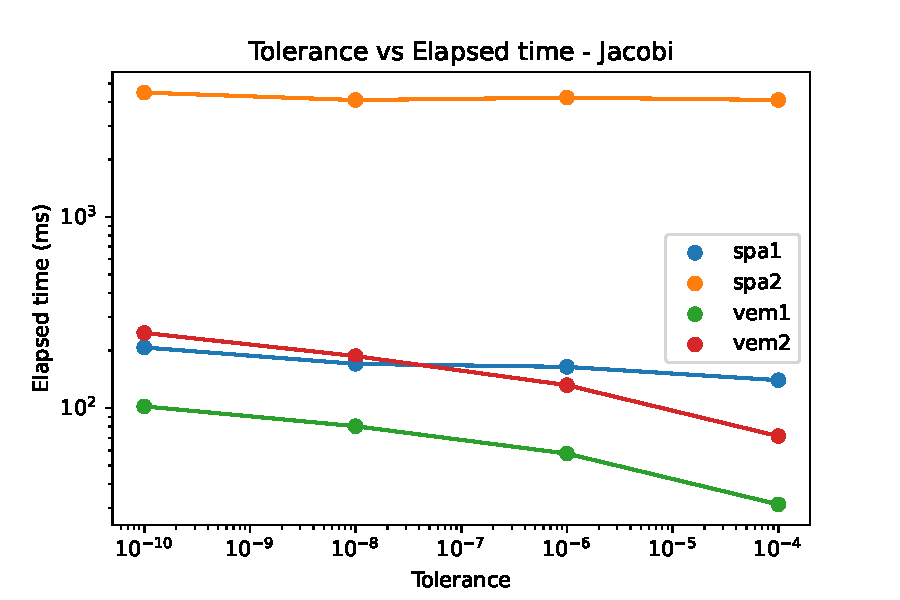
\includegraphics[width=0.40\textwidth]{figures/Tolerance vs Elapsed time/Difference between the 4 matrices on the same method/Jacobi.pdf} }}%
	\subfloat{{\includegraphics[width=0.40\textwidth]{figures/Tolerance vs Elapsed time/Difference between the 4 matrices on the same method/Conjugate Gradient.pdf} }}%
	\qquad
	\subfloat{{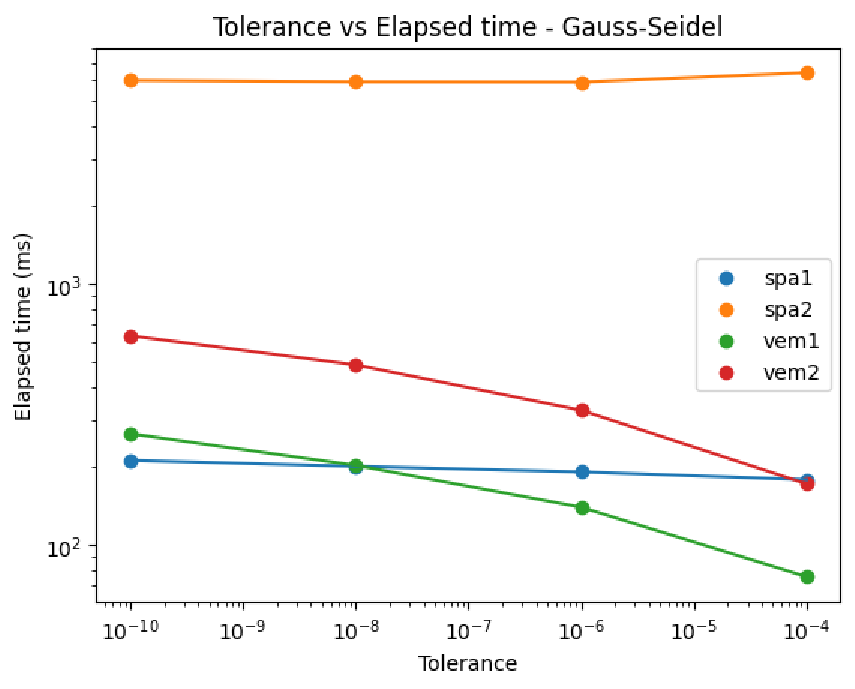
\includegraphics[width=0.40\textwidth]{figures/Tolerance vs Elapsed time/Difference between the 4 matrices on the same method/Gauss-Seidel.pdf} }}%
	\subfloat{{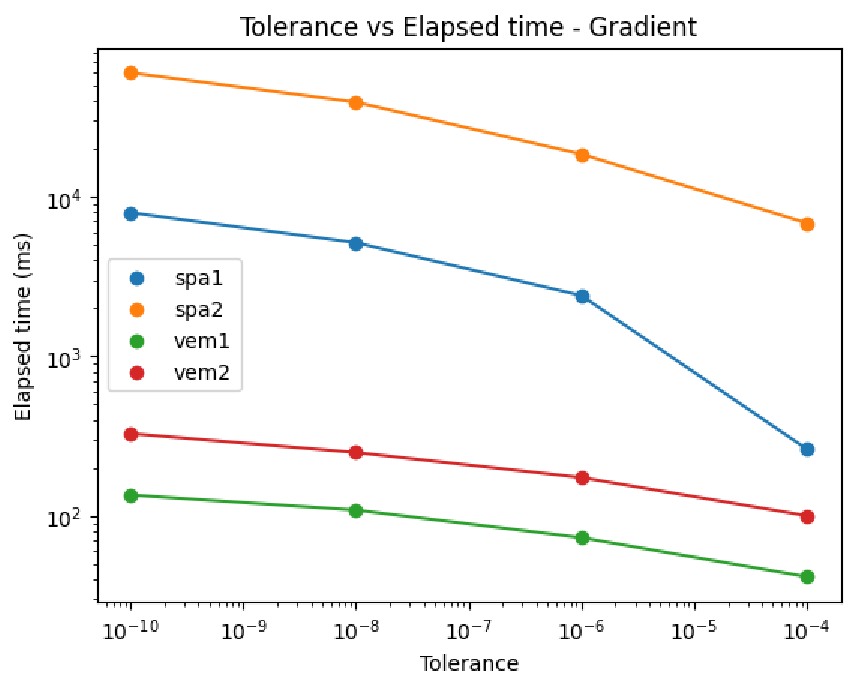
\includegraphics[width=0.40\textwidth]{figures/Tolerance vs Elapsed time/Difference between the 4 matrices on the same method/Gradient.pdf} }}%
	\caption{Grafici tolleranza / tempi rispetto i singoli metodi}%
	\label{fig:toltimemet}
\end{figure}
%Immagine tolerance-elapsedTime, spa1, difference between the 4 methods
%Immagine tolerance-elapsedTime, spa2, difference between the 4 methods

Nelle Figure \ref{fig:toltimemat} e \ref{fig:toltimemet} sono rappresentati i grafici relativi all'andamento del tempo rispetto alla tolleranza, raggruppati rispettivamente per matrice e per metodo.
Gauss Seidel è l'algoritmo che per le matrici relativamente dense, surclassa ogni altro metodo. Quando si passa a matrici estremamente sparse, come \path{vem1} e \path{vem2}, l'algoritmo che si comporta meglio sembra essere, invece, il gradiente coniugato.

Dai grafici si evince immediatamente che, all'aumentare della tolleranza, il tempo di esecuzione di ogni algoritmo tende a calare. Questa tendenza è più che ragionevole dato che, al calare della tolleranza, il criterio di arresto diventa più permissivo.
Tuttavia, è anche importante notare che, a differenza dell'errore relativo, il tempo di esecuzione dei vari metodi sembra poco sensibile sensible alla tolleranza selezionata; inoltre, l'andamento tra le due misure sembra dipendere pesantemente dal tipo di matrice, per ogni metodo. Questo potrebbe suggerire che ogni metodi funzionimeglio su un determinato tipo di matrice, anche se non abbiamo abbastanza dati per estrarre delle conclusioni. Questa osservazione è basata soprattutto dai grafici rappresentanti i tempi di Gauss-Seidel e di Jacobi: \path{vem1} e \path{vem2} sono matrici estremamente sparse, con una percentuale di elementi non nulli inferiore all'1\%, mentre \path{spa1} e \path{spa2} hanno una percentuale di elementi diversi da zero che si aggira attorno al 18\%: entrambi i metodi riescono ad abbassare visibilmente i tempi per le matrici molto sparse, mentre, nel caso della più dense, questo rimane più o meno invariato. Questa caratteristica, ovviamente, potrebbe dipendere anche da altri fattori non analizzati, come la qualità dei numeri presenti all'interno delle matrici.


%%%%%%%%%%%%%%%%%%%%%%%%%%%%%%%%%%%%%%%%%%%%%%%%%%%%%%%%%%%%%%%%%%%%%%%%%%%%%%%%%%%%%%%%%%%%%
%%%%%%%%%%%%%%%%%%%%%%%%%%%%%%%%%%%%%%%%%%%%%%%%%%%%%%%%%%%%%%%%%%%%%%%%%%%%%%%%%%%%%%%%%%%%%
%%%%%%%%%%%%%%%%%%%%%%%%%%%%%%%%%%%%%%%%%%%%%%%%%%%%%%%%%%%%%%%%%%%%%%%%%%%%%%%%%%%%%%%%%%%%%

%Immagine tolerance-elapsedTime, spa1, difference between the 4 matrixes on the same method
%Immagine tolerance-elapsedTime, spa2, difference between the 4 matrixes on the same method
%Immagine tolerance-elapsedTime, vem1, difference between the 4 matrixes on the same method
%Immagine tolerance-elapsedTime, vem2, difference between the 4 matrixes on the same method



